178. \begin{figure}[ht!]
\center{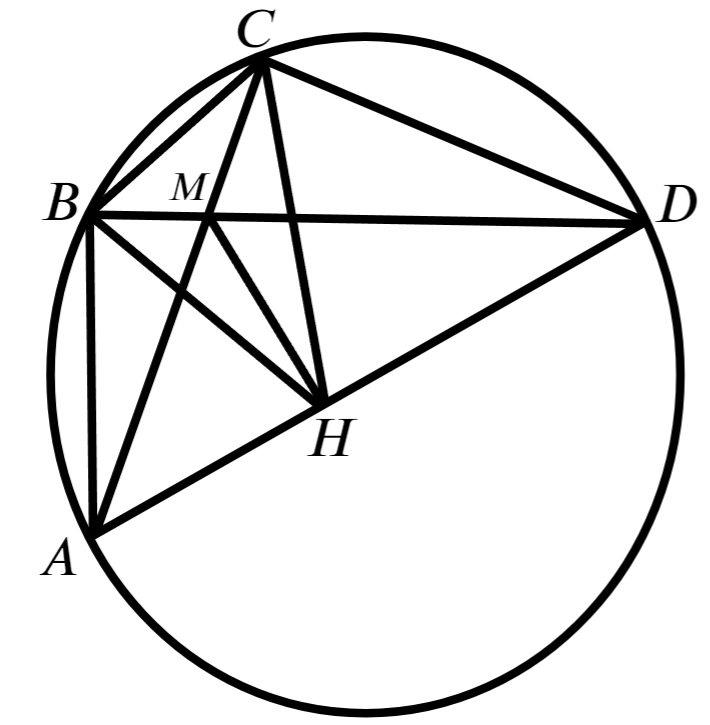
\includegraphics[scale=0.35]{g9-178.png}}
\end{figure}\\
Так как $AD$ --- диаметр окружности, то $ \angle ACD = 90^\circ.$ Поэтому в четырёхугольнике $HMCD$ сумма противоположных углов $\angle MCD$ и $\angle MHD$ равна $90^\circ+90^\circ=180^\circ$ и он является вписанным. Тогда $\angle MCH = \angle MDH = \angle BDA =  \angle BCA =  \angle BCM,$
то есть $CA$ --- биссектриса угла $BCH$ треугольника $BHC.$
Аналогично и $BD$ --- биссектриса угла $CBH$ треугольника $BHC.$ Значит, биссектрисы треугольника $BHC$ пересекаются в точке $M,$ поэтому она является центром его вписанной окружности, ч.т.д.\\
